\section{Двухуровневая оптимизация.}

\D{
    Двухуровневая оптимизация = задача оптимизации, содержащая
    другую задачу оптимизации в ограничениях.

    $$F(x_u, x_l) \to \min$$

    subject to:
    
    $$x_l \in \arg \min\{f(x_u, x_l) | g(x_u, x_l)\}$$

    $$G_j(x_u, x_l) \geq 0$$
}

\subsection*{Зачем нужна}

\begin{figure}[H]
    \centering
    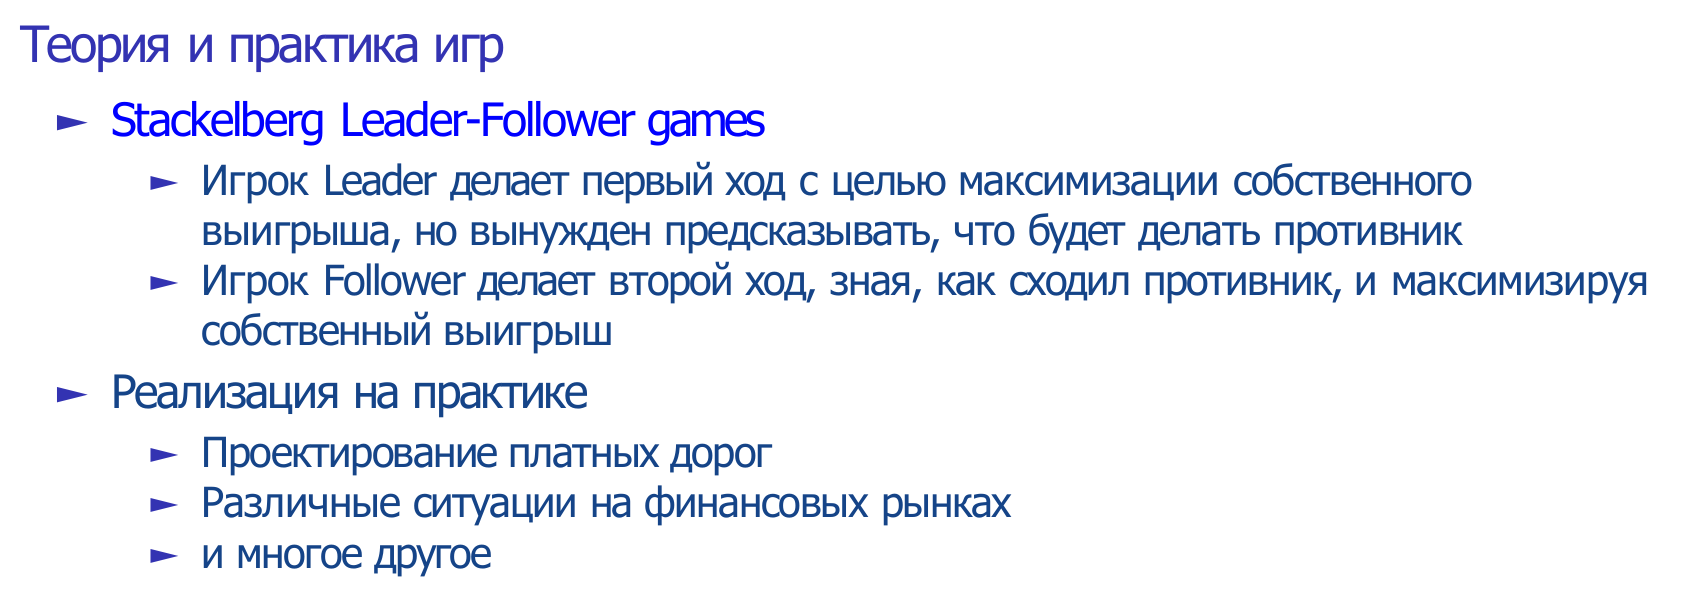
\includegraphics[width=0.8\linewidth]{images/65why.png}
    \caption{Зачем}
\end{figure}

А также:
\begin{itemize}
    \item Робастность и стабильность (оптимизация при условии стабильности решения)
    \item Структурная оптимизация: подбираем структуру + ее параметры
    \item Настройка параметров (алгоритма на задаче)
\end{itemize}

\subsection*{Проблемы}

\begin{figure}[H]
    \centering
    
\includegraphics[width=0.8\linewidth]{images/65pain.png}
    \caption{Боль}
\end{figure}

\subsection*{Методы решения}

\begin{itemize}
    \item Вложенная оптимизация: работает, но жрет много ресурсов.
    \item Условия Каруша-Куна-Таккера: условия оптимальности решения с ограничениями.
    (там всякая дичь про двойственную задачу => оно вам не надо)
    \item BLEAQ
    \item BLEMO
\end{itemize}

"Там все сложно, поэтому я вам ничего не расскажу" \textcopyright Simar
